% !TeX root = ../../../main.tex
\begin{figure}[htbp]
\begin{ChSixFloatBody}

    \begin{minipage}[t]{0.24\textwidth}
    \centering
    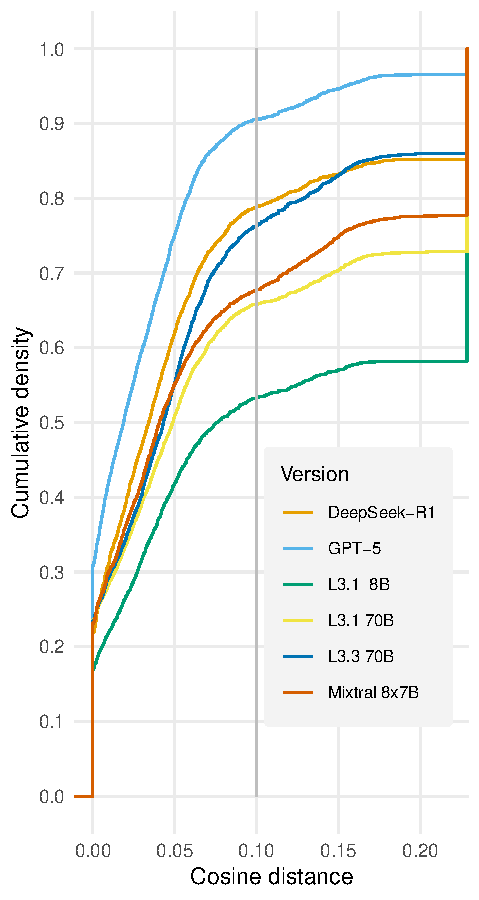
\includegraphics[width=\linewidth, page=1]{Chapters/chapter-06/images/figures/main_results_figures/figures_sepsis_40.pdf}
    \end{minipage}
    \hfill
    \begin{minipage}[t]{0.24\textwidth}
    \centering
    \includegraphics[width=\linewidth, page=2]{Chapters/chapter-06/images/figures/main_results_figures/figures_sepsis_40.pdf}
    \end{minipage}
    \begin{minipage}[t]{0.24\textwidth}
    \centering
    \includegraphics[width=\linewidth, page=3]{Chapters/chapter-06/images/figures/main_results_figures/figures_sepsis_40.pdf}
    \end{minipage}
    \begin{minipage}[t]{0.24\textwidth}
    \centering
    \includegraphics[width=\linewidth, page=4]{Chapters/chapter-06/images/figures/main_results_figures/figures_sepsis_40.pdf}
    \end{minipage}
    
    
    

\end{ChSixFloatBody}
\caption{Event match cumulative distribution function (left), concordance box-plots (middle left), 
    time discrepancy from the manual annotation timestamps among matched events, overall (middle right), and disaggregated by clinician annotator timestamp (time from presentation, right) for the \texttt{sepsis-40} dataset.}\ChSixFloatLabel{ch06:fig:time-disc}
\end{figure}